\chapter*{}

\textcolor{teal}{\centerline{\Huge{Probabilidad Y Estadística}}}


\begin{tikzpicture}
	\fill [left color=green!40, right color=red!50] (0,0) rectangle (11.5,.1);
	\end{tikzpicture}

\begin{figure}[H]
	\centering
	
\includegraphics[width=1\textwidth]{imagenes/hic-svnt-dracones.png}
\end{figure}



\begin{tikzpicture}
	\fill [left color=red!50, right color=green!40] (0,0) rectangle (11.5,.1);
	\end{tikzpicture}

\rightline{\textsf{\textit{\textcolor{purple!70}{Ignacio Vallés Oriola}}}}

\newpage
$\quad$
\newpage
$\quad$



\begin{figure}[H]
	\centering
	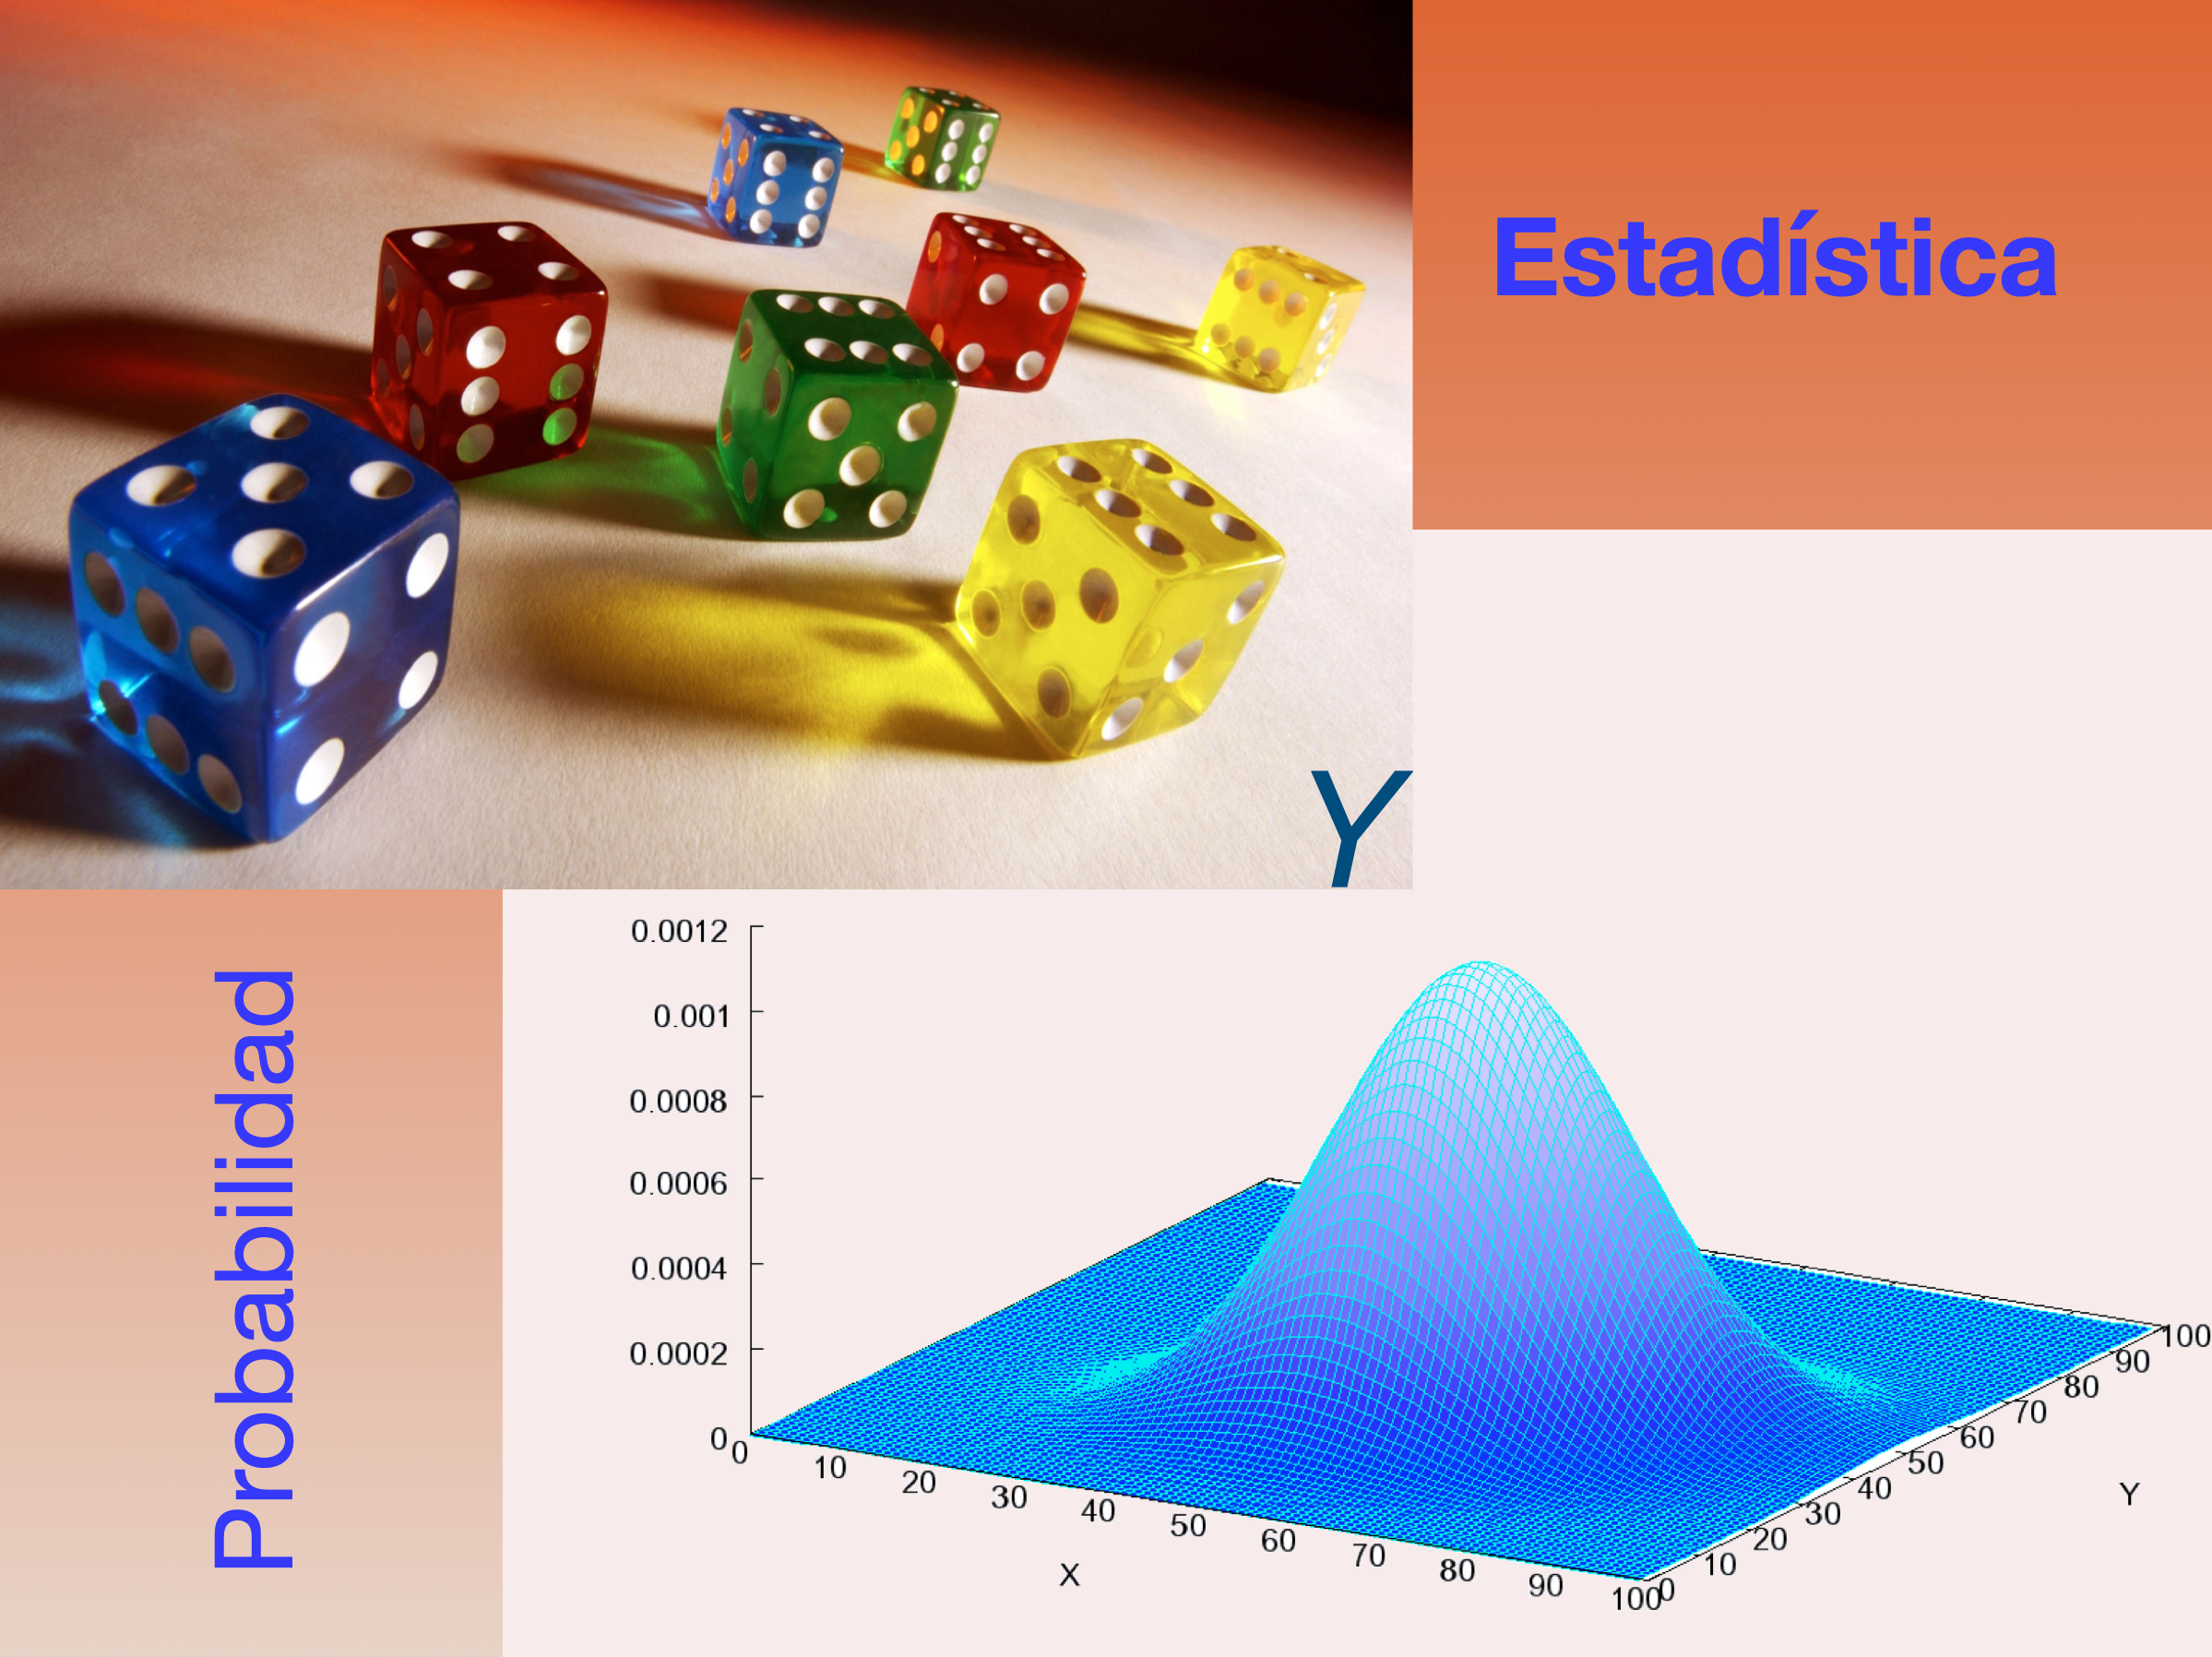
\includegraphics[width=1\textwidth]{imagenes/imagenes00/T01IM01.png}
\end{figure}

\vspace{2 cm}

\begin{quotation} \begin{quotation}
\noindent 
\begin{large}
\begin{itemize}
\item I - Estadística descriptiva
	\begin{itemize}
	\item 1 - Estadística descriptiva
	\item 2 - Distribuciones bidimensionales: Correlación y Regresión lineal
	\end{itemize}
\item II - Probabilidad
	\begin{itemize}	
	\item 3 - Cálculo de Probabilidades
	\item 4 - Distribuciones de probabilidad
	\end{itemize}
\item III - Estadística inferencial
	\begin{itemize}
	\item 5 - Distribuciones muestrales. Estimación
	\item 6 - Contraste de Hipótesis. 
	\end{itemize}
\end{itemize}
\end{large}
\end{quotation} \end{quotation}

\newpage %*****************************************************


\section{?`Qué es la Estadística?}

	
\begin{tikzpicture}
	\fill [left color=black!30, right color=white] (0,0) rectangle (11.5,.1);
	\end{tikzpicture}

Podemos decir que la Estadística es la \emph{herramienta} que se utiliza cuando se quiere estudiar un hecho, el que sea, y no se conocen las leyes que lo rigen. 

En estos casos lo único que se puede hacer es \emph{observar el fenómeno} o suceso de interés y \emph{tomar datos}, y luego analizar esos datos y ver si tienen relación con otras variables, si se comportan de alguna forma especial... 

La Estadística consiste en todo eso, recoger los datos, estudiarlos, analizarlos y sacar conclusiones. Y basándonos en las observaciones, a veces seremos capaces de proponer una ley que explique o que al menos describa el comportamiento del suceso. 

Como herramienta al servicio de otras ciencias la Estadística aparece en todas partes, Física, Química, Biología... y también ciencias sociales, Economía, Sociología, Psicología...  Hasta en Lingüística se usa la estadística para determinar, por ejemplo, las letras más frecuentes en los textos de una lengua.  

\textbf{Un poco de historia...} 

Las antiguas civilizaciones, como la egipcia, la china y la azteca, ya hacían estadísticas sobre el número de personas que vivían en las ciudades, normalmente para organizar el pago de impuestos y el ejército. En general a lo largo de toda la historia los gobiernos y dirigentes de las distintas naciones han procurado disponer de datos sobre la población con fines organizativos. 

La Estadística como ciencia experimentó un gran avance gracias al desarrollo de la Matemáticas, en especial de la \emph{Teoría de la Probabilidad}, cuyas bases no fueron establecidas hasta el siglo XVII por los matemáticos franceses Pierre de \emph{Fermat} y Blaise \emph{Pascal}. ¿`Y qué tiene que ver la Probabilidad con la Estadística? ¡`Mucho! Hemos dicho que la Estadística es un instrumento para el estudio de un fenómeno cuando no se conocen que leyes lo rigen, y si hay fenómenos que no están regidos por leyes eso son los fenómenos aleatorios. Y la base matemática para el estudio estadístico de los fenómenos aleatorios la proporciona la Teoría de la Probabilidad. 

\begin{footnotesize}
\begin{quotation}
	\textcolor{gris}{INSTITUTOS NACIONAL DE ESTADÍSTICA. \textsf{INE}}
	
	\textcolor{gris}{https://www.ine.es/explica/explica.htm}
	
\end{quotation}
\end{footnotesize}

\begin{multicols}{2}
\begin{figure}[H]
	\centering
	
\includegraphics[width=.3\textwidth]{imagenes/imagenes00/T01IM03.png}
\end{figure}
\begin{figure}[H]
	\centering
	
\includegraphics[width=.3\textwidth]{imagenes/imagenes00/T01IM02.png}
\end{figure}
\end{multicols}

La estadística se divide en dos partes, la \emph{Estadística Descriptiva} que se encarga de la recogida de datos de un proceso aleatorio, clasificarlos, representarlos gráficamente y reducirlos a números estadísticos y la \emph{Estadística Inferencial} que se encarga de deducir consecuencias a partir de los datos proporcionados por la estadística descriptica y hacer predicciones. Para ello se basa en la \emph{Teoría de las probabilidades}.


\section{Estructura de este libro}




 
La estructura del libro se presenta del siguiente modo:

\vspace{5mm} %***************************
\begin{definition}
. De esta manera aparecerán las definiciones.

%\textbackslash begin\{definition\}.....\textbackslash end\{definition\}	
\end{definition}

\vspace{5mm} %***************************
\begin{theorem}
. En estos recuadros aparecerá la teoría: teoremas, propiedades, ...

%\textbackslash begin\{theoreme\} ..... \textbackslash end\{theoreme\}	
\end{theorem}

\vspace{5mm} %***************************
\begin{example}
.	Estos recuadros están reservados a los ejemplos que ilustran los distintos apartados.

%\textbackslash begin\{example\}.......\textbackslash end\{example\}	
\end{example}


\vspace{5mm} %***************************
\begin{myalertblock}{Ampliación}
	Aquí aparecerán las ampliaciones de la teoría.
\end{myalertblock}


\vspace{5mm} %***************************
\begin{myexampleblock}{Curiosidades}
	Reservamos este cuadro para     las curiosidades relacionadas con el tema que se esté tratando.
\end{myexampleblock}


\vspace{5mm} %***************************
\begin{myblock}{Resumenes}
	Al final de cada tema aparece un. resumen del mismo.
\end{myblock}


\vspace{5mm} %***************************
\begin{ejemplo}
\begin{ejre}
	Así pondremos los ejercicios del tema.
	
%\textbackslash begin\{ejemplo\} \textbackslash begin\{ejre\} .........   \textbackslash end\{ejre\} \textbackslash end\{ejemplo\}
\end{ejre}
Las soluciones a los ejercicios del tema aparecerán fuera del recuadro (dentro de ellos en los que he llamado `ejercicios resueltos').
\end{ejemplo}

Los ejercicios propuestos con solución que acompañan a todos los temas aparecen sin ningún tipo de resalte.

\vspace{5mm} %***************************
\begin{destacado}
Párrafo destacado: reservamos esta forma de resaltar para hacer incapié sobre determinados aspectos importantes del tema.

%\textbackslash begin\{destacado\}	........ \textbackslash end\{destacado\}	
\end{destacado}


\section{Guía de lectura}

\textbf{Tema 1. Estadística descriptiva unidimensional}

\begin{adjustwidth}{50pt}{25pt}
En este capítulo se explican los conceptos básicos de la estadística descriptiva: tablas, gráficos y parámetros estadísticos: de centralización, de posición, de dispersión y de forma.

Para finalizar, se presenta el coeficiente de variación de Pearson para la comparación entre distribuciones estadísticas distintas. Se introduce el concepto de  ``tipificación de la variable''.
\end{adjustwidth}

\textbf{Tema 2. Distribuciones bidimensionales. Correlación y regresión lineal}

\begin{adjustwidth}{50pt}{25pt}
En el tema se estudia la correlación lineal entre dos variables estadísticas y, en su caso (que así lo indique el diagrama de dispersión y que el coeficiente de correlación sea, en valor absoluto, próximo a la unidad), encontrar la recta que mejor se ajusta a la nube de puntos, la recta de regresión.

Se hacen predicciones con las dos rectas de regresión haciendo hincapié en que la mayor fiabilidad de las interpolaciones.

Se menciona la recta de Tukey como alternativa a la de regresión ante la presencia de \emph{outliers} y, como ampliación, se habla de las correlaciones exponencial y potencial, ambas no lineales.
\end{adjustwidth}

\textbf{Tema 3. Probabilidad}

\begin{adjustwidth}{50pt}{25pt}
Después de introducida el álgebra de los sucesos de experimentos aleatorio se dan varias definiciones de probabilidad: a posteriori o frecuencialista y a priori o regla de Laplace. A continuación se enuncia la definición axiomática de Kolmogorov.

Seguimos com la definición de probabilidad condicionada y los teoremas de la probabilidad total y de Bayes. Este tema, por su interés y dificultad, se ve con más detenimiento y se acompaña de gran cantidad de ejemplos y ejercicios resueltos y propuestos con solución.
\end{adjustwidth}

\textbf{Tema 4. Distribuciones de probabilidad}

\begin{adjustwidth}{50pt}{25pt}
Las distribuciones de probabilidad son idealizaciones matemáticas de las distribuciones estadísticas. En el presente tema se analizan detalladamente las distribuciones de probabilidad más importantes: la binomial (para variable aleatoria discreta) y la normal (para variable aleatoria continua).

Como distribuciones de variable aleatoria discreta se analizan también la distribución uniforme, la de Bernouilli y la de Poisson. Para variable continua se estudian, someramente, la distribución uniforme continua y la exponencial.

En la distribución normal se estudi el uso de tablas para la normal típica o standard N(0,1) y la ``tipificación de la variable'' para cualquier distribución normal $N(\mu,\sigma)$.

El tema termina con el estudio de la aproximación de la binomial por la normal y la correspondiente ``corrección por continuidad''.

Este tema se acompaña de gran cantidad de ejemplos y ejercicios resueltos y propuestos con solución.

\end{adjustwidth}

\textbf{Tema 5. Distribuciones muestrales. Estimación}

\begin{adjustwidth}{50pt}{25pt}
Comenzamos con la definición y cálculo de los intervalos característicos en una distribución normal típica y en una normal cualquiera, que usaremos más tarde en la estimación de parámetros por intervalos.

Estudiamos la distribución de las medias muestrales y analizamos el teorema central del límite. Se aprende a hacer estimaciones puntuales y por intervalos de confianza de la media de la población (conocida una muestra) y de la media de una muestra (conocida la población). Se hace notar la relación entre el nivel de confianza, el error máximo admisible y el tamaño de la muestra.

Como ampliación, vemos la distribución de la diferencia de medias de dos muestras.

El tema acaba analizando la distribución de la proporción y haciendo estimaciones para la proporción de una población y de una muestra.

Este tema se acompaña de gran cantidad de ejemplos y ejercicios resueltos y propuestos con solución.
\end{adjustwidth}

\textbf{Tema 6. Contraste de hipótesis}

\begin{adjustwidth}{50pt}{25pt}

En el estudio del contraste de hipótesis se estudian los elementos que la componen así como la metodología general de su aplicación, teniendo en cuenta los dos tipos de posibles errores en que se puede caer.

Estudiamos el contraste de hipótesis para la media de un población y para la proporción de una población. Como ampliación, vemos el contraste de hipótesis para la diferencia de medias de dos poblaciones.

Este tema se acompaña de gran cantidad de ejemplos y ejercicios resueltos y propuestos con solución.
\end{adjustwidth}

\textbf{Apéndices}

\begin{adjustwidth}{50pt}{25pt}
A - ``Ideas básicas de la teoría de conjuntos'': analizamos el álgebra de Boole como sistema lógico de amplia aplicación en probabilidad.

B - ``Combinatoria. Técnicas de conteo'': principio de multiplicación, principio del palomar, permutaciones, variaciones y combinaciones 8con y sin repetición). Estrategia de los diagramas de árbol. Números combinatorios, triangulo de Tartaglia y binomio de Newton.

C - ``Tablas de las distribuciones Binomial y Normal''.

D - ``El problema del borracho''. Analizamos en este apéndice el famoso problema cuyo enunciado dice: \emph{
``Un borracho parte de un farol dando pasos de igual longitud hacia ambos lados. ?`Cuál es la probabilidad de que después de $N$ pasos vuelva al farol?''
}
\end{adjustwidth}






\section{Acerca de este libro}

El presente libros, colección de apuntes, contempla la parte de estadística de los temarios de bachillerato. Junto a los otros dos, ``Cálculo infinitesimal (avanzado) para bachillerato'' y ``Álgebra lineal y geometría (avanzadas) para bachillerato'', este ``Probabilidad y estadística (avanzadas) para bachillerato'' contemplan todo el temario actual de matemáticas de este nivel de enseñanza.

Es cierto que falta la parte de ``Programación lineal'' que haré en una nueva pequeña entrega.

La confección de estos textos es fruto de una larga experiencia como profesor de matemáticas de secundaria y para ello me he basado en mis más de treinta años de docencia  y en la de tantos autores que han contribuido a la explicación de estos conceptos a multitud de alumnos. He usado también apuntes y problemas de libros de texto de segundo de bachillerato así como apuntes y ejercicios encontrados en la web y pruebas de acceso a la universidad de distintas comunidades autónomas. Gracias a todos sus autores por su inestimable ayuda para la confección de estos textos que espero que sirva a alguien y que escribo libre de todo tipo de derechos. 


\vspace{5mm}
\centering{
\fcolorbox{black}{fondoblau}{
\parbox{0.95\textwidth}{
	\textit{Este material es un conjunto de apuntes personales que comparto gratuitamente en la red. Se agradecería la comunicación de la detección de cualquier error.}
}}}
\justify

\emph{Este documento se comparte bajo licencia `Attribution-NonCommercial 4.0 International (CC BY-NC 4.0)'}


\begin{multicols}{2}
\begin{figure}[H]
	\centering
	
\includegraphics[width=.4
	\textwidth]{imagenes/imagenes00/licencia.png}
\end{figure}
\begin{figure}[H]
	\centering
	
\includegraphics[width=.3
	\textwidth]{imagenes/firma.png}
\end{figure}
\end{multicols}





